In questo appendice, si mostrano brevemente i grafici che non sono stati inseriti direttamente nel Sezione \ref{sec:alpha}, dove sono stati discussi gli effetti che ha il parametro $\alpha$ nella scelta dei costi dei cammini.
In particolare, nelle Figure \ref{figapx:alpha1} e \ref{figapx:alpha2} sono riportati i grafici contenenti i costi dei cammini scelti durante la simulazione (aggregati ogni 100 \textit{step} della simulazione).

\begin{figure}
	\begin{tabular}{cc}
		\subfloat[Effetto di un valore del parametro $\alpha$ pari a $10^{-4}$ nella scelta della cella obiettivo in base al costo del cammino.]{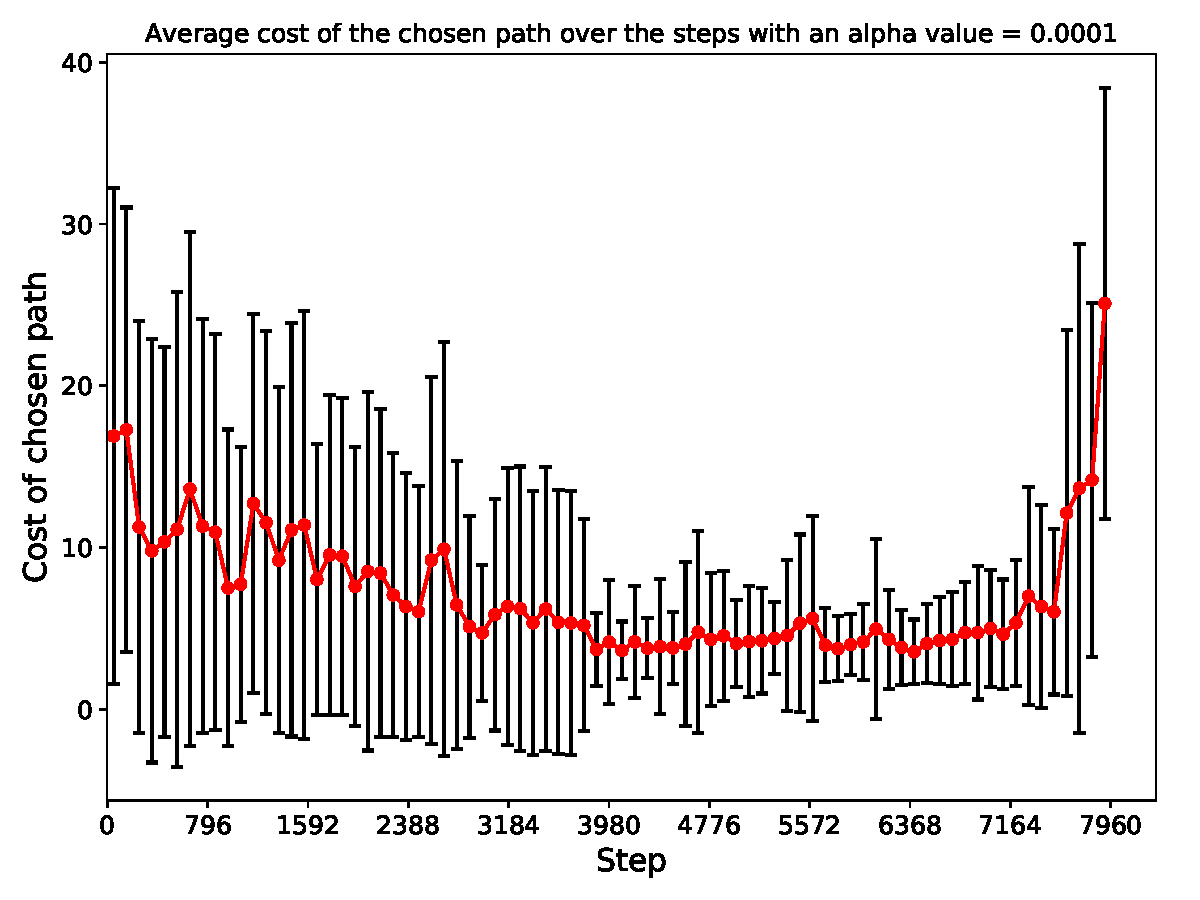
\includegraphics[width = .5\textwidth]{images/alpha_results/cost_alpha_0_0001}} &
		\subfloat[Effetto di un valore del parametro $\alpha$ pari a 0.0005 nella scelta della cella obiettivo in base al costo del cammino.]{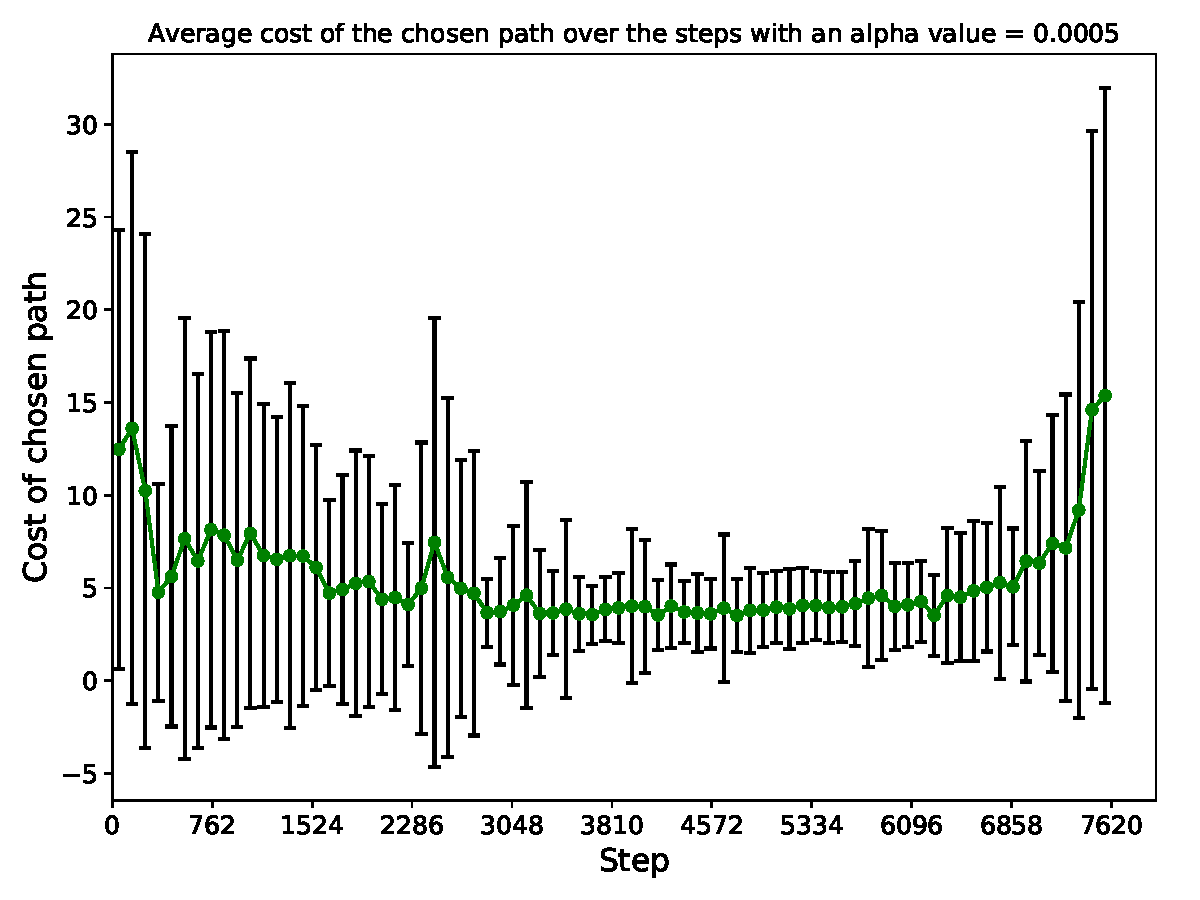
\includegraphics[width = .5\textwidth]{images/alpha_results/cost_alpha_0_0005}}\\
		\subfloat[Effetto di un valore del parametro $\alpha$ pari a 0.001 nella scelta della cella obiettivo in base al costo del cammino.]{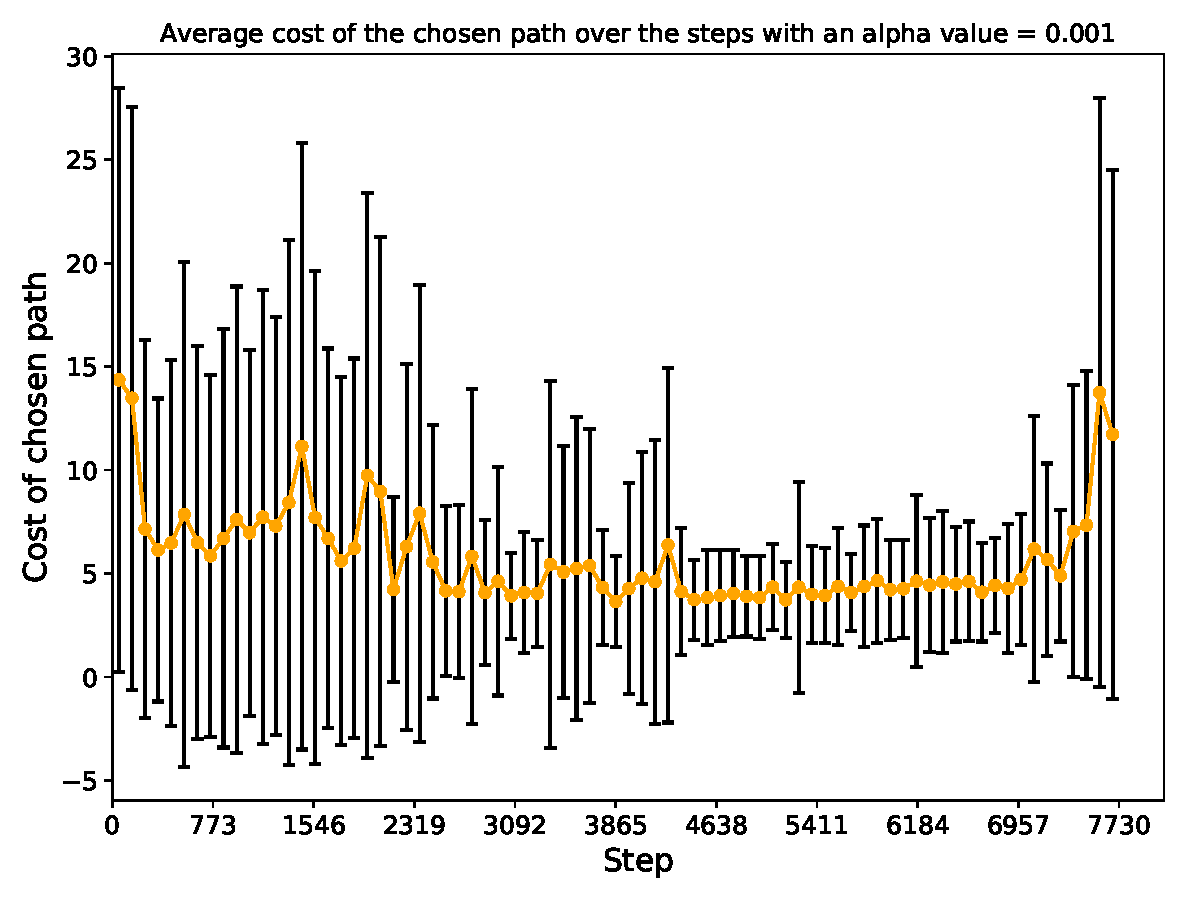
\includegraphics[width = .5\textwidth]{images/alpha_results/cost_alpha_0_001}} &
		\subfloat[Effetto di un valore del parametro $\alpha$ pari a 0.005 nella scelta della cella obiettivo in base al costo del cammino.]{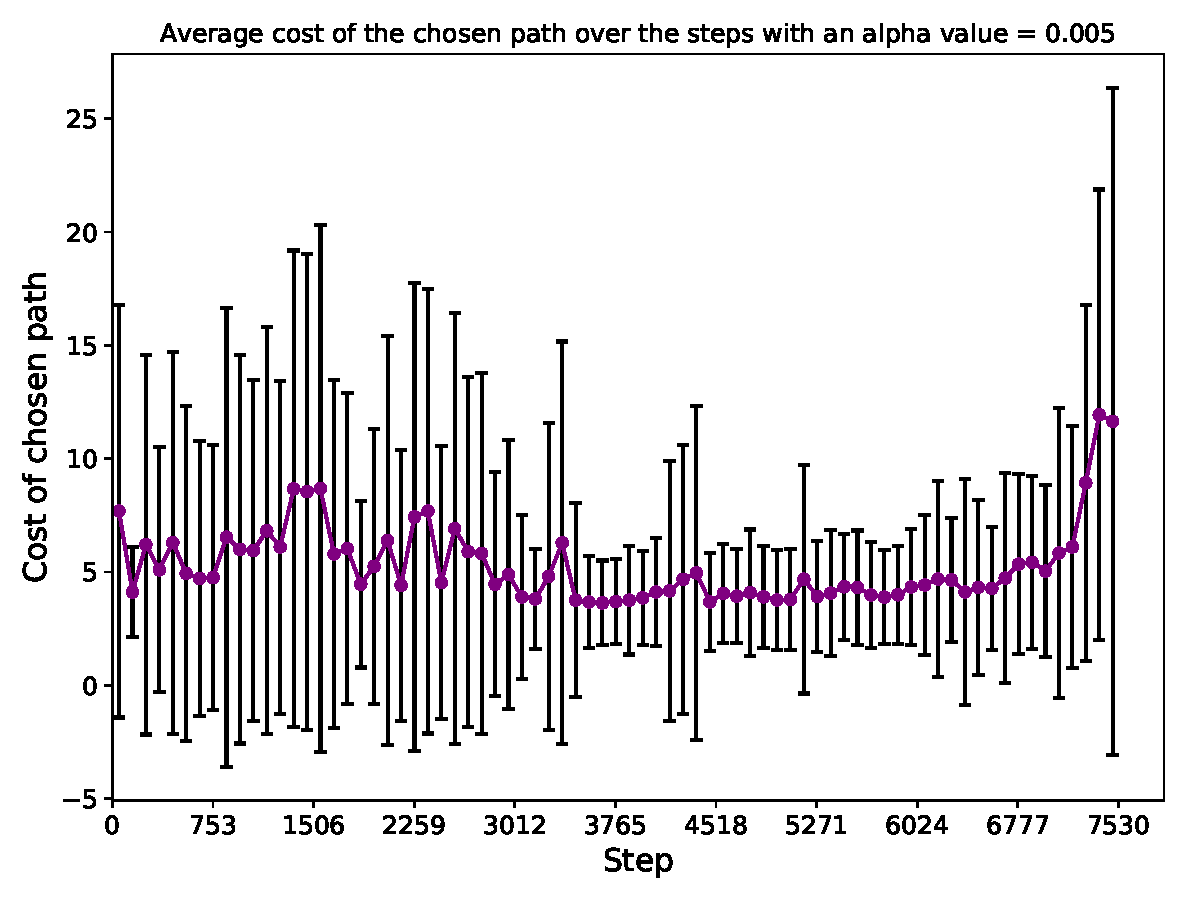
\includegraphics[width = .5\textwidth]{images/alpha_results/cost_alpha_0_005}}\\
	\end{tabular}
	\caption{In colore si denota la media dei costi dei cammini per raggiungere la cella scelta, i valori sono stati calcolati aggregando le scelte effettuate durante intervalli di 100 \textit{step}; in nero gli \textit{errorbar} relativi alla media determinati dalla deviazione standard.}
	\label{figapx:alpha1}
\end{figure}

\begin{figure}
	\begin{tabular}{cc}
		\subfloat[Effetto di un valore del parametro $\alpha$ pari a 0.05 nella scelta della cella obiettivo in base al costo del cammino.\label{sfig:alpha0.05}]{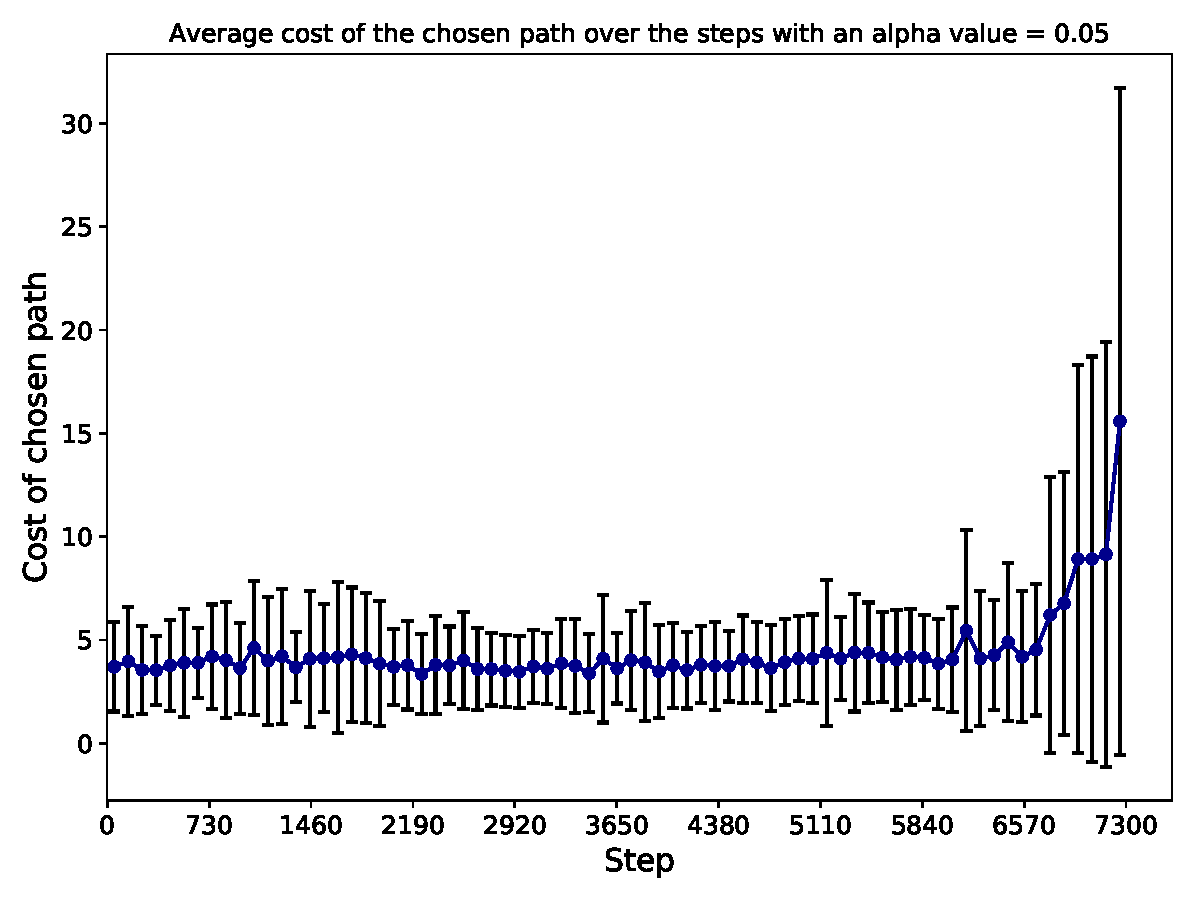
\includegraphics[width = .5\textwidth]{images/alpha_results/cost_alpha_0_05}} &
		\subfloat[Effetto di un valore del parametro $\alpha$ pari a 0.1 nella scelta della cella obiettivo in base al costo del cammino.]{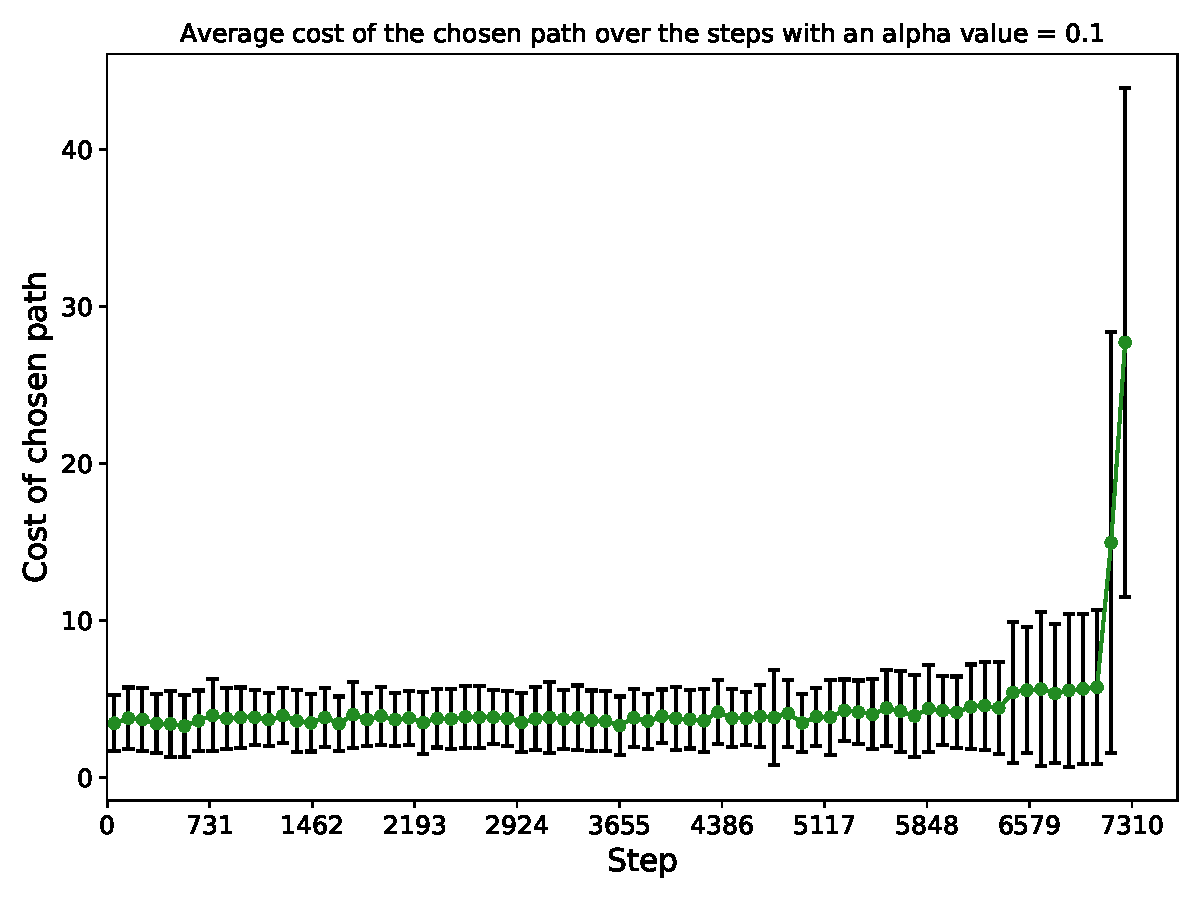
\includegraphics[width = .5\textwidth]{images/alpha_results/cost_alpha_0_1}}\\
	\end{tabular}
		\centering
		\subfloat[Effetto di un valore del parametro $\alpha$ pari a 1 nella scelta della cella obiettivo in base al costo del cammino.]{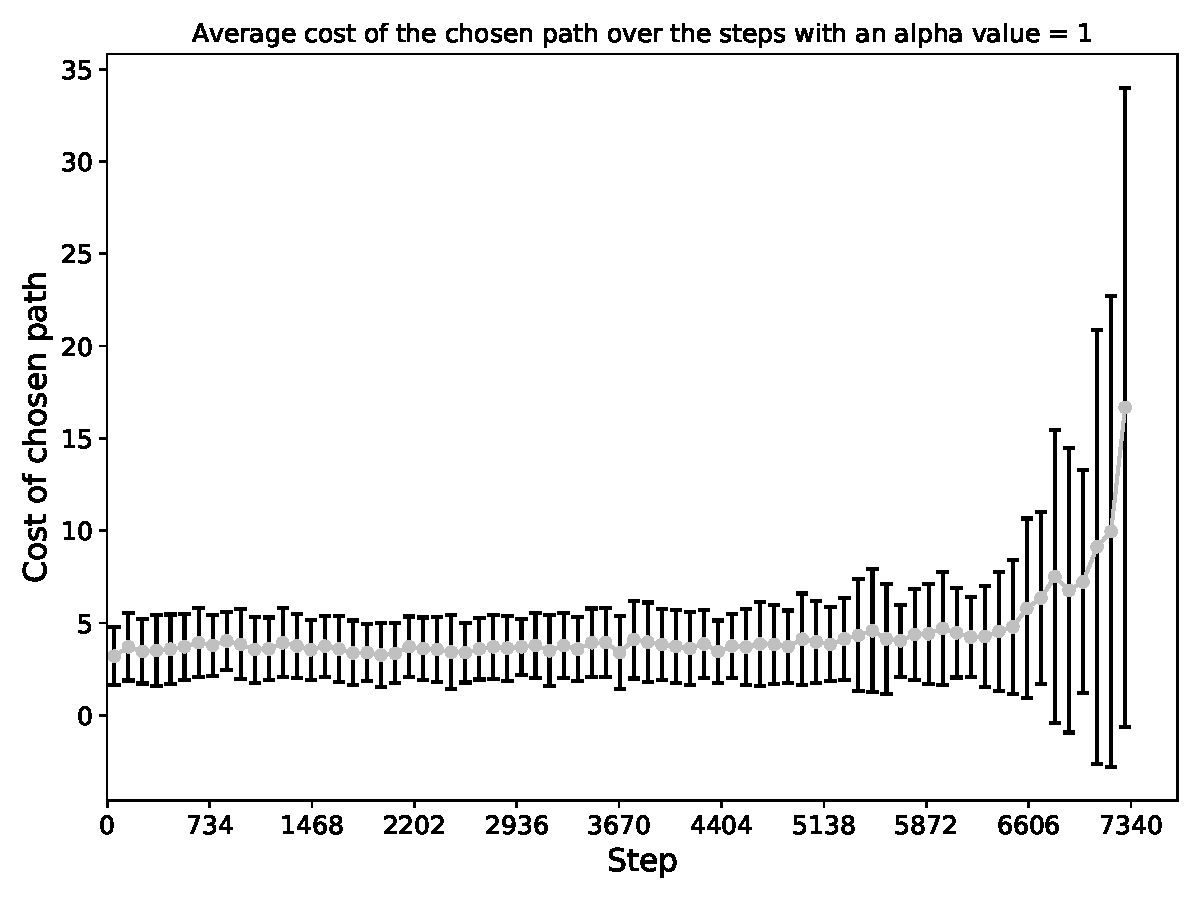
\includegraphics[width = .5\textwidth]{images/alpha_results/cost_alpha_1}}
	\caption{In colore si denota la media dei costi dei cammini per raggiungere la cella scelta, i valori sono stati calcolati aggregando le scelte effettuate durante intervalli di 100 \textit{step}; in nero gli \textit{errorbar} relativi alla media determinati dalla deviazione standard.}
	\label{figapx:alpha2}
\end{figure}